\documentclass{beamer}
% Try the class options [notes], [notes=only], [trans], [handout],
% [red], [compress], [draft] and see what happens!

% \usepackage{definitions}
\usepackage[british]{babel}
\usepackage{color, soul}
\usepackage{tikz}

%% tikz tricks
% \tikzset{onslide/.code args={<#1>#2}{%
%   \only<#1>{\pgfkeysalso{#2}} 
% }}

\pdfinfo{
        /Title (cim)
        /Creator (LaTeX)
        /Producer (pdflatex)
        /Author (szerzo)
        /CreationDate (datum)
	/Subject (tema)
}


\mode<article> % only for the article version
{
  \usepackage{fullpage}
  \usepackage{hyperref}
}
\mode<presentation>
{
  \usetheme[left,width=0.65in,height=0.55in]{Kolozsvar}
  \setbeamercovered{transparent}
  \setbeamertemplate{navigation symbols}{}
  \setbeamertemplate{footline}%
     {\vspace*{-1.4em}\hspace*{0.66in}\textbf{\insertframenumber/\inserttotalframenumber}\newline\vspace*{0.4em}}
		\setbeamerfont{block title}{size=\larger} % RELSIZE -- html-sizes 
		\usefonttheme{professionalfonts}
		\setbeamercolor{math text}{fg=green!30!red!30!brown}
		\setbeamercolor{normal text in math text}{parent=math text}
}

\setbeamercovered{dynamic}

% The following info should normally be given in you main file:
\title[Smart Office]{Smart Office}

%
\author{Hunor Ördög, Norbert-Raymond Pap, István-Lehel Balázs}
%
\institute[UBB Cluj-Napoca]{
  Department of Mathematics and Informatics\\
  Babe{\c{s}}--Bolyai University, Cluj-Napoca}
%
\date{2025 January}


\begin{document}

\frame{\maketitle}

\mode<presentation>
{
  % \begin{frame}
  %   \frametitle{Talk structure}
  % \tableofcontents
  % \end{frame} 

  % \AtBeginSection[]
  {
      \begin{frame}<beamer>{Contents}
        % \tableofcontents[currentsection,currentsubsection,hideothersubsections]
        \tableofcontents
      \end{frame}
    }
}

%%%%%%%%%%%%%%%%%%%%%%%%%%%%%%%%%%%%%%%%%%%%%%%%%%%%%%%%%%%%%%%%%%%%%%


\section[Introduction]{Introduction}

\begin{frame}{Introduction}
  \begin{itemize}
      \item IoT application that collects real-time sensor data and displays it on a web interface.
      \item Monitoring environmental conditions such as light, humidity, temperature, motor activity.
      \item \textbf{Features:}
      \begin{itemize}
          \item Sensor data visualization in real-time.
          \item Motor control via the web interface.
          \item Historical data retrieval for analysis.
      \end{itemize}
  \end{itemize}
\end{frame}

\section[Workflow]{Workflow}

\begin{frame}{Workflow Overview}
  \begin{itemize}
      \item \textbf{Data Collection:}
      \begin{itemize}
          \item Arduino Uno collects sensor data (e.g., temperature, humidity).
          \item Communication with NodeMCU via \textbf{SPI protocol}.
      \end{itemize}
      \item \textbf{Web Hosting:}
      \begin{itemize}
          \item NodeMCU hosts a web page accessible to users.
      \end{itemize}
      \item \textbf{Data Transmission:}
      \begin{itemize}
          \item Sensor data is sent to the webpage every second.
      \end{itemize}
      \item \textbf{Data Persistence:}
      \begin{itemize}
          \item Data is also saved to Firebase.
      \end{itemize}
      \item \textbf{Historical Data Retrieval:}
      \begin{itemize}
          \item On user request, older data is fetched from Firebase based on specified dates.
      \end{itemize}
  \end{itemize}
\end{frame}

\section[Data Format]{Data Format}

\begin{frame}{Firebase Data Format}
  \hspace*{2.6em}
  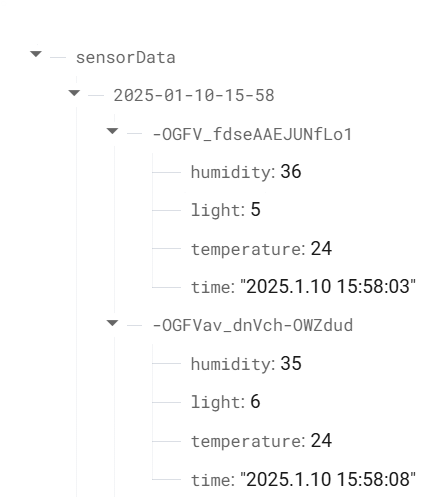
\includegraphics[scale=0.7]{fig/fb_format.png}
\end{frame}

\section[Data Chart]{Data Chart}


\begin{frame}{Data Display on Chart}
  % \hspace*{.3em}
  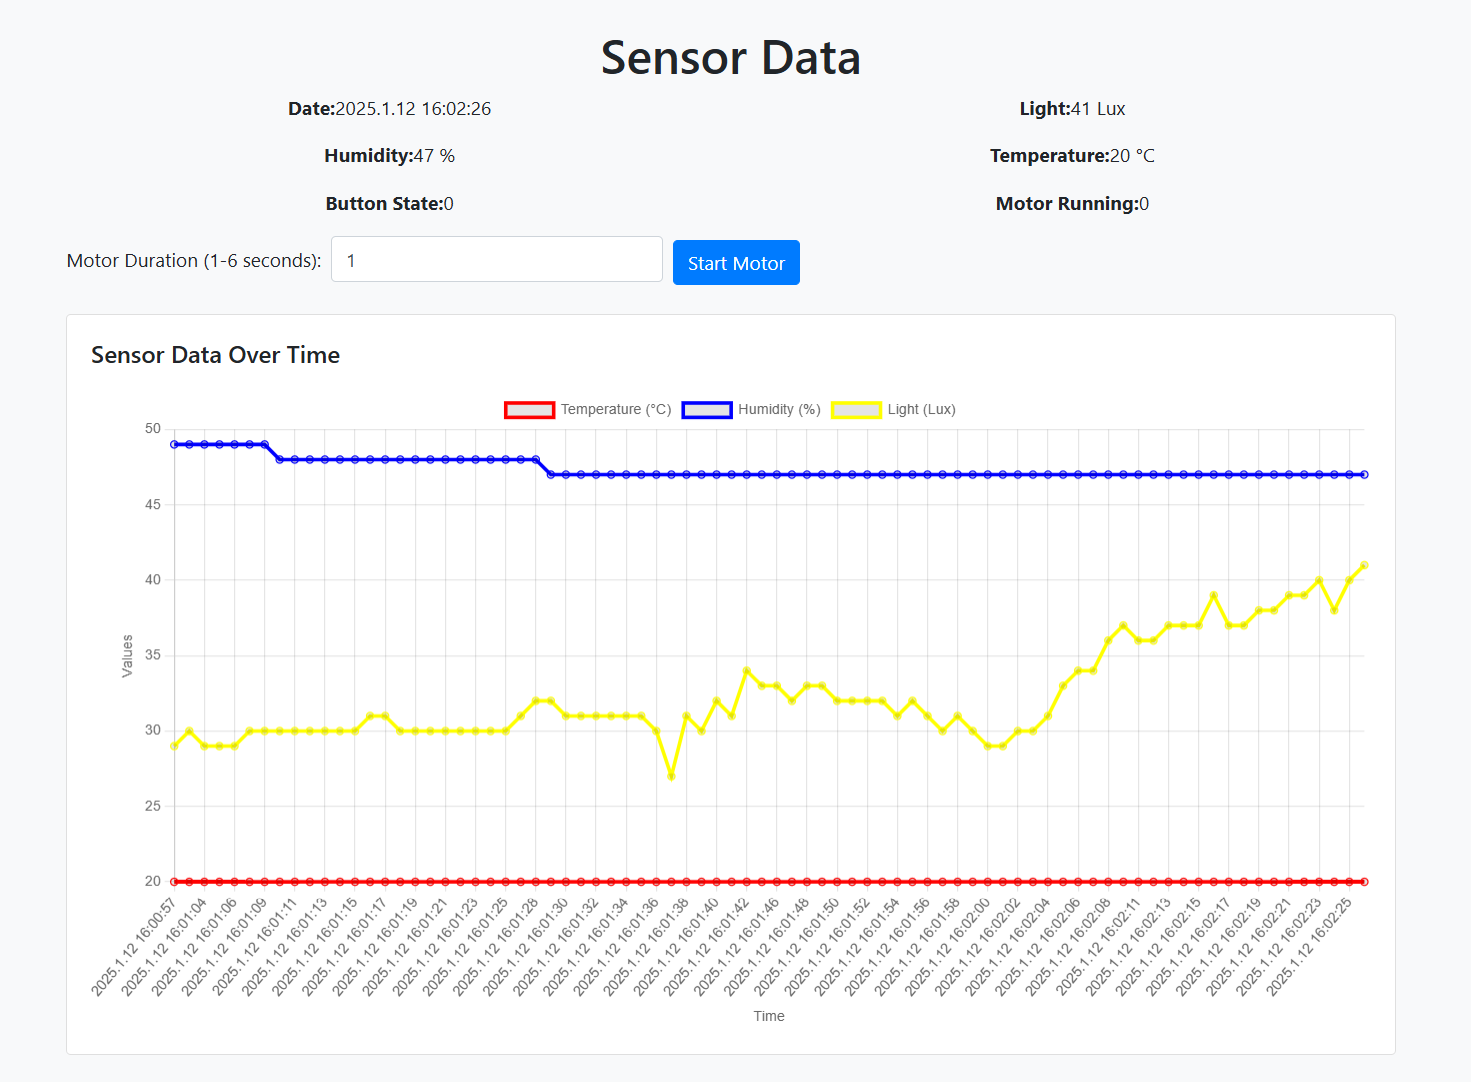
\includegraphics[scale=0.32]{fig/senschart.png}
\end{frame}

\end{document}
